% !TeX root = ../report.tex
% !TeX spellcheck = en-US
% !TeX encoding = UTF-8
\chapter{CONTROLLER DESIGN}\label{chap:controller design}


\section{CRAWLER}
% Describe the current working of the crawler Use diagram and crawler pictures

% Describe the choices that we need to make

% Strategy

% Peripherals

\section{STRATEGY DECISION}\label{sec:strategy decision}
%describe the decision matrix with uncertainties
\import{resources/}{strategy_decision_matrix}

%plot and motivate the choice

\section{PERIPHERALS}\label{sec:peripherals}

\subsection{COMMUNICATION}\label{sec:communication}

\subsubsection{WIRELESS}\label{sec:wireless}

\subsubsection{UMBILICAL}\label{sec:umbilical}


\subsection{LOCALIZATION}\label{sec:localization}

\subsubsection{IMU SENSOR}\label{sec:imu sensor}

\subsubsection{DEPTH SENSOR}\label{sec:depth sensor}
% pressure sensor environment

\subsubsection{SATELLITE DRONES}\label{sec:Cooperative localization}

% Use GIB text and image compare with kleunen echoes from the deep

\subsection{PROPULSION SENSORS}\label{sec:propulsion sensors}
% torque measurement with the use of a current sensor
% rotational measurement

\subsection{PRODUCTION SENSORS}\label{sec:production sensors}
% Pressure sensor
% flow sensor

\section{KALMAN FILTER DESIGN}

In Chapter~\ref{sec:cpp} it became evident that an accurate estimation of a crawlers position and heading is needed
such that it can perform its tasks using \gls{acr-CPP} algorithms. Because it is not possible to use \gls{acr-GPS} in an
underwater environment, due to the dampening of electric and magnetic fields in water, which was described in
Section~\ref{sec:em}, an alternative localization method had to be found. Chapter~\ref{sec:coverageunderuncertainty}
describes \gls{gls-Kalman-filter} as the industry de-facto. Position estimation for the control will therefore be
performed with this algorithm.

A design for an \gls{gls-Kalman-filter} is proposed, using a common array of sensors, such as: \gls{gls-accelerometer},
\gls{gls-gyroscope}, \gls{gls-magnetometer} and a \gls{gls-pressure-sensor}. The workings for each of these are
discussed Section~\ref{sec:sensors} and the component selection was made in Section~\ref{sec:strategy decision}. The
crawler is actuated by, changing the rotational speed of the individual \gls{gls-Archimedes-screw}s.

\begin{RoyalFigure}[!htb, label=fig:kalman process]{PROPOSED KALMAN FILTER}
	\begin{tikzpicture}[auto, node distance=2cm,>=latex', align=center, inner sep=5mm, thick,scale=0.8, everynode/.style={scale=0.6}]
		\node[block] (controller) {Controller};
		\node[block, right of=controller, xshift=7.5cm] (actuator) {Actuator};
		\node[block, right of=actuator, xshift=1cm] (process) {Process};
		\node[block, below of=actuator] (current) {Current};
		\node[block, below of=current] (encoder) {Encoder};
		\node[block, below of=encoder] (gyro) {Gyroscope};
		\node[block, below of=gyro] (acc) {Accelerometer};
		\node[block, below of=acc] (mag) {Magnetometer};
		\node[block, below of=mag](press) {Pressure \\ sensor};
		\node[block, left of=current, xshift=-3cm] (slip predict) {Slip \\ Predict};
		\node[block, left of=slip predict, xshift=-1cm, fill=RoyalLightGrey] (soil param) {Soil \\ Parameters};
		\node[block, below of=soil param, fill=RoyalLightGrey] (geo param) {Geometry \\ Parameters};
		\node[block, below of=slip predict, yshift=-8cm] (kalman) {Unscented \\ Kalman \\ filter};
		\node[output, right of=process](output) {};
		\node[blockdashedwhite, label=below:{\large \textbf{Measurement}},fit={(current) (acc) (mag) (press)} ] (measurement) {};
		\node[blockdashedwhite, label=below:{\large \textbf{microcontroller}},fit={(controller) (kalman) (slip predict)} ] (microcontroller) {};

		\draw[-latex] (controller) -- (actuator) node[midway,above,yshift=-5mm] {\gls{sym-u}};
		\draw[-latex] (actuator) -- (process) node[midway,above,yshift=-5mm] {$ \gls{sym-tau} $, $ \gls{sym-omega} $ };
		\draw (actuator.east) -| ($(current.east)+(0.5,0)$);
		\draw[-latex] ($(current.east)+(0.5,0)$) -- (current.east);
		\draw[-latex] ($(current.east)+(0.5,0)$) |- (encoder.east);
		\draw[-latex] (process.east) -- (output);
		\draw[-latex] (current.west) -- (slip predict.east)  node[midway,above,yshift=-5mm] { $I$ };
		\draw[-latex] (soil param.east) -- (slip predict.west);
		\draw (geo param.east) -| ($(slip predict.west)-(0.5,0)$);
		\draw[-latex] (slip predict.south) -- (kalman.north) node[midway,above,xshift=-3mm] { $u_k^{\prime}$ };
		\draw[-latex] (kalman.west) -| (controller.south) node[midway,above,yshift=-5mm,xshift=1.5cm] { $\gls{sym-x_k}$} ;
		\draw[-latex] (press.west) -- (kalman.east)  node[midway,above,yshift=5mm] { $\gls{sym-y_k}$ };
		\draw (encoder.west) -| ($(kalman.east)+(1,0)$);
		\draw (gyro.west) -| ($(kalman.east)+(1,0)$);
		\draw (acc.west) -| ($(kalman.east)+(1,0)$);
		\draw (mag.west) -| ($(kalman.east)+(1,0)$);
		\draw[-latex] ($(process.east)+(0.5,0)$) |- (gyro.east);
		\draw[-latex] ($(process.east)+(0.5,0)$) |- (acc.east);
		\draw[-latex] ($(process.east)+(0.5,0)$) |- (mag.east);
		\draw[-latex] ($(process.east)+(0.5,0)$) |- (press.east);
		\node[right of=process, xshift=1.5mm,yshift=0.5mm] (x) {$x$};
	\end{tikzpicture}
\end{RoyalFigure}

Where the speed of an  \gls{gls-Archimedes-screw} driven crawler is a direct function of the pitch of its vanes. But
this only applies if there is no horizontal soil failure under the screws. Such a phenomena is called slip. It consist
of a period in time where the screws turn, but generate no forwarding force. Leading to an inaccurate estimation for the
new predicted state. Due to the geometry of an \gls{gls-Archimedes-screw}, this slip coexist with an bulldozer effect
created by the vanes acting as a shovel in the soil. This will lead to an increase in torque. It is proposed that by
measuring the required torque of the drive train, a prediction can be made how much slip has occurred, leading to a
better estimation of the future state-vector \gls{sym-x_kt+1}. This behavior and the mathematical model will be
discussed in more detail in Section~\ref{sec:motion model}. Figure~\ref{fig:kalman process} shows the interaction and
connectivity of the various components that server as the input and output of the proposed filter.

Since the physical processes for movement of a crawler are non-linear and the ``basic'' \gls{gls-Kalman-filter},
described in Section~\ref{sec:basic Kalman filter} is limited to linear assumptions, the proposed
\gls{gls-Kalman-filter} is of the Unscented variant. The \gls[first]{acr-UKF} uses a deterministic sampling technique
known as \gls[first]{acr-UT}. This technique picks a minimal set of sample points, also known as sigma points, around
the mean. The sigma points are then propagated through the non-linear function, from which a new mean and covariance
estimate are then formed.

\subsection{STATE REPRESENTATION}\label{sec:state representation}

\citet{bahr_cooperative_2009} states that, the most generic case of a vehicle operating in 3D Euler-space, such as a
crawler, consist of a vector of variables comprised of a vehicle's pose and orientation. The pose is its position in a
(global) reference frame \( \left[\gls{sym-x} ~\gls{sym-y} ~\gls{sym-z}\right]^T \). While  its orientation is given in
Euler angles \( \left[\gls{sym-phi_c} ~\gls{sym-psi_c} ~\gls{sym-theta_c}\right]^T \). The pose vector at time
\gls{sym-t} is then \( \gls{sym-x_k} = \left[\gls{sym-x} ~\gls{sym-y} ~\gls{sym-z} ~\gls{sym-phi_c} ~\gls{sym-psi_c}
\gls{sym-theta_c}\right]^T \), which will be denoted as  \gls{sym-x_k} for the remainder of this paper. Beside the pose,
the state vector can also contain the first and second derivatives of the pose vector.

\begin{RoyalFigure}[!htb, label=fig:staterepentation]{STATE REPRESENTATION}
		\resizebox{0.6\textwidth}{!}{
			\begin{tikzpicture}
			\node[anchor=south west,inner sep=0] (image) at (0,0) {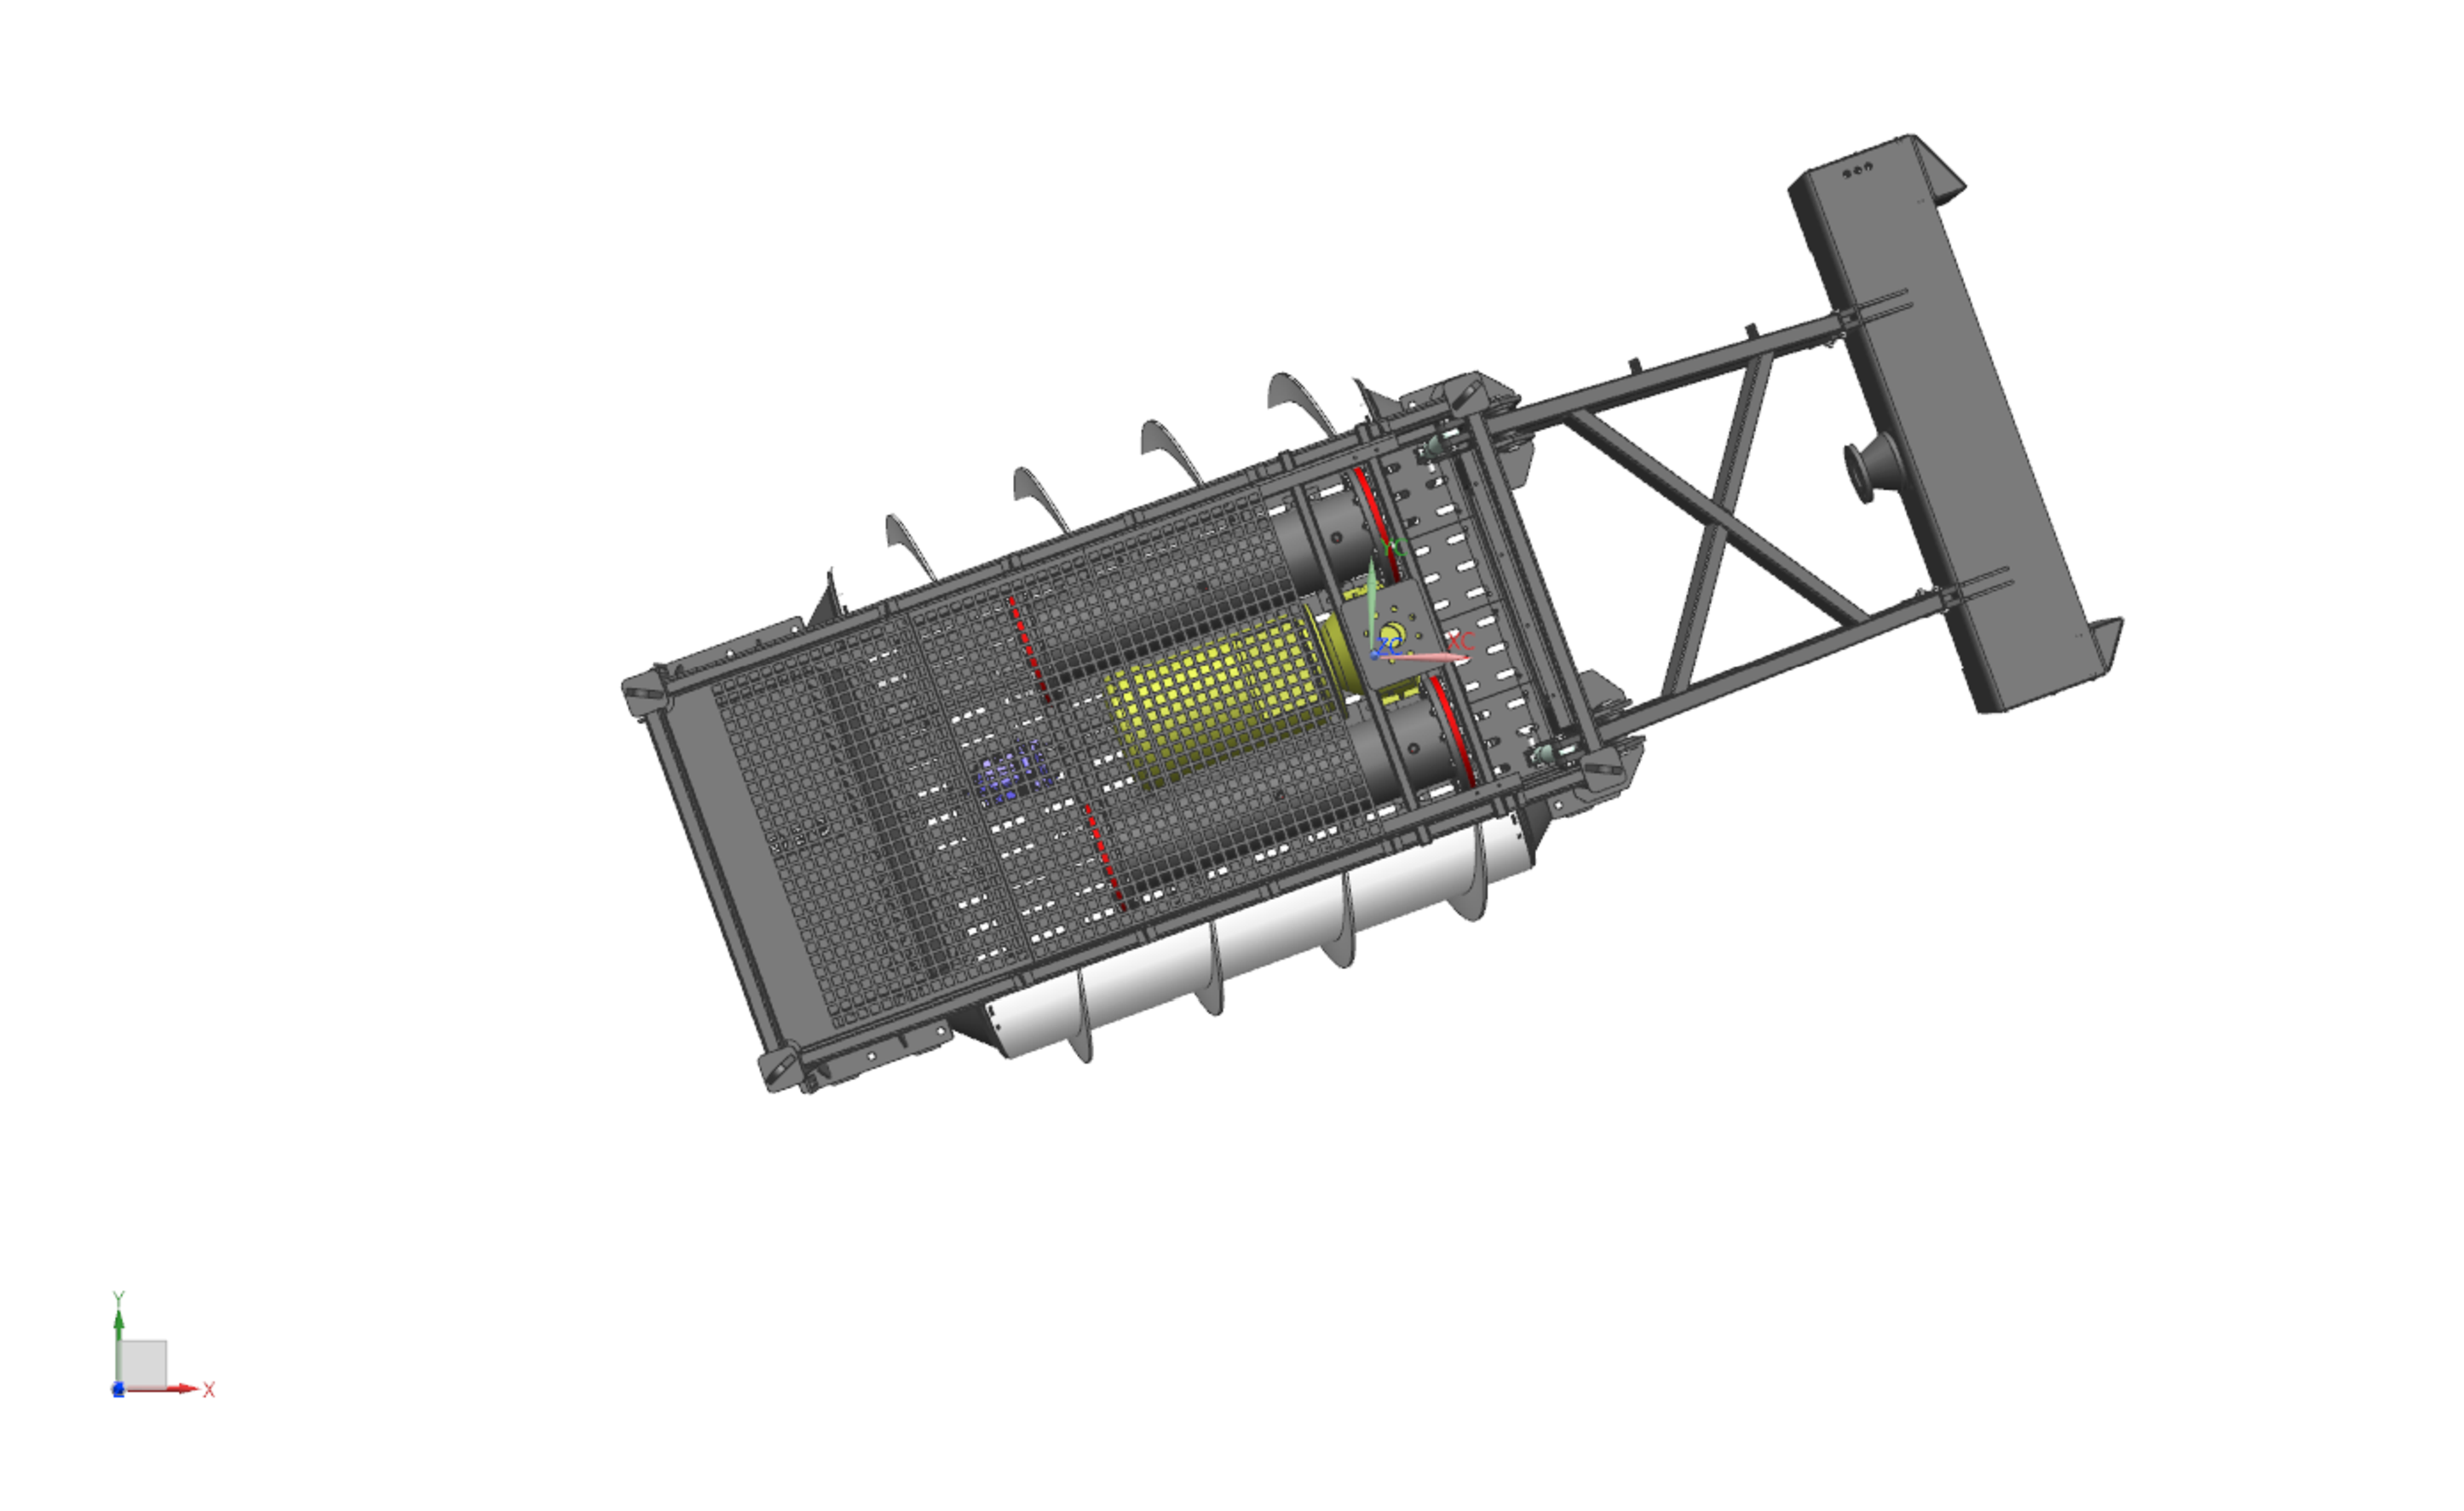
\includegraphics[width=.9\textwidth, trim=2 2 2 2,clip]{dredgebottop.pdf}};
			\node[draw, line width=0.75mm, inner sep=0, circle, minimum size=0.75cm,align=center] (xyz) at (0.6,0.6) {\\ {\huge z}};
			\node[anchor=south west,inner sep=0] (y) at ([shift=(90:8cm)]xyz.center) {{\huge $ y $}};
			\node[anchor=south west,inner sep=0] (x) at ([shift=(00:8cm)]xyz.center) {{\huge $ x $}};
			\node[anchor=south west,inner sep=0] (v_xyz) at (7.9,4.8) {};
			\node[anchor=south west,inner sep=0] (v_xyz_text) at (8,4.2) {$ z^V $};
			\node[anchor=south west,inner sep=0] (v_y) at (7.9,8) {};
			\node[anchor=south west,inner sep=0] (v_x) at (12,4.8) {};
			\node[anchor=south west,inner sep=0] (heading) at ([shift=(22.5:5cm)]v_xyz) {$ x^V $};
			\node[anchor=south west, inner sep=0] (perp_heading) at ([shift=(112.5:3cm)]v_xyz) {$ y^V $};

			\node[anchor=south west,inner sep=0] (vec) at (3,1.5) { $ \gls{sym-x_k} =\left[\gls{sym-x},\gls{sym-y},\gls{sym-z}\right] $ };

			\draw[-latex, line width=0.75mm] (xyz.center) to (x);
			\draw[-latex, line width=0.75mm] (xyz.center) to (y);
			\draw[-latex,red, line width=0.5mm] (xyz.center) to (v_xyz);
			\draw[-latex,green, line width=0.5mm] (v_xyz.center) to (heading);
			\draw[-latex,green, line width=0.5mm] (v_xyz.center) to (perp_heading);
			\draw[dashed, line width=0.25mm] (v_xyz.center) to (v_y.center);
			\draw[dashed, line width=0.25mm] (v_xyz.center) to (v_x.center);

			\draw[latex-latex, line width=0.25mm] ([xshift=2cm]v_xyz.center) arc (0:22.25:2cm) node [right,pos=0.5] {$ \gls{sym-psi_c} $};
			\draw[latex-latex, line width=0.25mm,rotate=22.5] ([xshift=-1cm, yshift=-0.5cm]heading) arc (-120:150:0.20cm and 0.55cm) node [above,pos=0.85] {$ \gls{sym-phi_c} $};
			\draw[latex-latex, line width=0.25mm,rotate=112.5] ([xshift=-1cm, yshift=-0.3cm]perp_heading) arc (-120:150:0.2cm and 0.55cm) node [above,pos=0.65] {\gls{sym-theta_b}};

			\end{tikzpicture}}
\end{RoyalFigure}

\subsubsection{2D OR 3D}

\citet{bahr_cooperative_2009} proposes the following simplification; They state that all submersible vehicles are
outfitted with a pressure sensor which allows them to determine their absolute depth with high accuracy and a high
update rate. As a result all underwater navigation systems are only used to resolve the 2D position and all underwater
vehicle related localization problems are stated in 2D. Which allows for a simplified state vector \( \gls{sym-x_k} =
\left[\gls{sym-x} ~\gls{sym-y} ~\gls{sym-phi_c} ~\gls{sym-psi_c} ~\gls{sym-theta_c}\right]^T \).

This simplification does not hold for crawlers or \gls{acr-AUV} that change in depth in any other direction then
collinear with the earths gravitational axis. Since this crawler moves over irregular terrain, any pitch or roll will
result in a gravitational force that also consist of components along the x-axis and / or y-axis. Which would then be
interpreted as movements in the 2D x-y space. This coupled with an unreliable pressure-sensor reading due to
disturbance of sediment from the sea bed during dredging operations, as described in Section~\ref{sec:pressure sensor},
means the the state representation should be in 3D Euler space, as is shown in figure~\ref{fig:staterepentation}.

\subsubsection{QUATERNIONS}

Because the \gls{acr-UKF} is executed on a embedded device, with limited resources, all rotational translations are
calculated with the help of \gls{gls-quaternion}s. Which make use of the same concept as complex numbers, except of
using one imaginary axis, there are three. Just as complex numbers are very useful in describing a rotation in a
two-dimensional plane, \gls{gls-quaternion}s are highly efficient in a three-dimensional space. They are also immune to
\gls{gls-gimbal-lock}ing. The exact workings are outside of the scope of this thesis, but for those readers which are
interested, a good explanation is given by \citet{3blue1brown_quaternions_2018} and can be found
at~\url{www.youtube.com/watch?v=d4EgbgTm0Bg}. A \gls{gls-quaternion}s is represented as a single column matrix with four
rows, consisting  of a real valued magnitude and three imaginary components for the axes \(\gls{sym-q} =
\left[\gls{sym-q_s} ~\gls{sym-q_x} ~\gls{sym-q_y}  ~\gls{sym-q_z} \right]^T \), Where the \gls{sym-q_s} is used to
normalize the \gls{gls-quaternion}, this keeps the error from accumulating. It is important to note that
\gls{gls-quaternion}s are \gls{gls-non-commutative}, thus the order in which they are applied matters to the outcome of
the rotation.

\subsection{MOTION MODEL}\label{sec:motion model}

It is important to evaluate the effects of control inputs \( \gls{sym-u_k} \) on the pose vector \( \gls{sym-p_k} =
[\gls{sym-x}, \gls{sym-y}, \gls{sym-z}]^T \) such that \( \gls{sym-p_kt_1} \) can be predicted. Since the
continuous-time model for the vehicle state's speed and rate can be described as:

\begin{equation}\label{eq:motionmodel}
	\gls{sym-p_kt_1} = f(\gls{sym-x_k},\gls{sym-u_k})
\end{equation}

The function \( f(\cdot) \) in equation~\ref{eq:motionmodel} can be very complex and is usually non-linear, it has to take
into account all external forces that can influence the movement of the crawler. According to
\citet{bahr_cooperative_2009} the more complex the model, the more accurately it can represent the vehicle dynamics and
provide a better prediction of the future pose, but obtaining such a model requires detailed knowledge of the structure
as well as the parameters listed below. All of which influence movement and sensor reading:
\begin{itemize}
	\setlength\itemsep{0mm}
	\item Shape of the crawler\footnote{\label{c} Constant parameter}\footnote{\label{used} Used in the model}
	\item Size of the crawler\footnotemark[\getrefnumber{c}]\footnotemark[\getrefnumber{used}]
	\item Weight of the crawler\footnotemark[\getrefnumber{c}]\footnotemark[\getrefnumber{used}]
	\item Buoyancy of the crawler\footnotemark[\getrefnumber{c}]\footnotemark[\getrefnumber{used}]
	\item Actuators (pumps, motors etc.) and their behavior, such as vibrations
	\item Forces exerted on the crawler due to fluid transportation through the floating line
	\item Forces exerted on the crawler due to the buoyancy of the floating line
	\item Forces exerted on the crawler from the umbilical
	\item Operating environment
	\begin{itemize}
		\setlength\itemsep{0mm}
		\item Properties of the soil bed \cite{lotman_applicable_2009};\footnotemark[\getrefnumber{used}]
		\begin{itemize}
			\setlength\itemsep{0mm}
			\item Density\footnotemark[\getrefnumber{used}]
			\item Cohesion\footnotemark[\getrefnumber{used}]
			\item Skin friction\footnotemark[\getrefnumber{used}]
		\end{itemize}
		\item Temperature
		\item Salinity
		\item Current
		\item Medium through which maneuver (mixture of water and soil)
	\end{itemize}
	\item Configuration of the propulsion system:
	\begin{itemize}
		\setlength\itemsep{0mm}
		\item Track variant\footnotemark[\getrefnumber{used}] \cite{lotman_applicable_2009}
		\begin{itemize}
			\item Length\footnotemark[\getrefnumber{c}]\footnotemark[\getrefnumber{used}]
			\item Distance between grouser plates\footnotemark[\getrefnumber{c}]\footnotemark[\getrefnumber{used}]
			\item Width of the track\footnotemark[\getrefnumber{c}]\footnotemark[\getrefnumber{used}]
			\item Height of the grouser plate\footnotemark[\getrefnumber{c}]\footnotemark[\getrefnumber{used}]
		\end{itemize}
		\item Archimedes screw variant\footnotemark[\getrefnumber{used}] \cite{van_der_zee_prediction_2009}
		\begin{itemize}
			\setlength\itemsep{0mm}
			\item Length\footnotemark[\getrefnumber{c}]\footnotemark[\getrefnumber{used}]
			\item Diameter\footnotemark[\getrefnumber{c}]\footnotemark[\getrefnumber{used}]
			\item \gls[first]{acr-SWR}\footnotemark[\getrefnumber{c}]\footnotemark[\getrefnumber{used}]
			\item Number of helices\footnotemark[\getrefnumber{c}]\footnotemark[\getrefnumber{used}]
			\item Pitch angle\footnotemark[\getrefnumber{c}]\footnotemark[\getrefnumber{used}]
			\item Vane height\footnotemark[\getrefnumber{c}]\footnotemark[\getrefnumber{used}]
			\item Front bulldozer angel\footnotemark[\getrefnumber{c}]\footnotemark[\getrefnumber{used}]
			\item slip\footnotemark[\getrefnumber{used}]
		\end{itemize}
	\end{itemize}
\end{itemize}

Not all parameters shown above, have the same impact on the future state representation. Since calculations on a complex
model require more processing power, only parameters with a substantial influence will be used. It is assumed that the
biggest influences are drag-forces, due to movement in a fluidium and the interaction with the Archimedes screw in the
silt layer. These will in all likelihood have a bigger impact than other operating parameters. Forces exerted on the
crawler due to a current, floating lines, and actuators are --- for now --- deemed to be a magnitude smaller and can
be ignored.

During travel between two points, it is preferred to minimize travel time. Which is usually achieved by moving at the
fastest sustainable speed. The propulsion system which acts on the submerged soil bed is governed by a lot of
interactions on the system as a whole. Which were listed in section~\ref{sec:motion model}. The crawler is propelled by
an Archimedes screw. A proven technology for land based vehicles. Especially in rough, impassable terrain. They have
shown reliable operations, superior traction capabilities and they can be used as a buoyancy body. Typical working
territories for Archimedes driven are dredge deposit sites and swamps \citet{lotman_deep_2011}.

\begin{RoyalFigure}[!htb, label=fig:archimedes_drive_train]{ARCHIMEDES DRIVE TRAIN}
	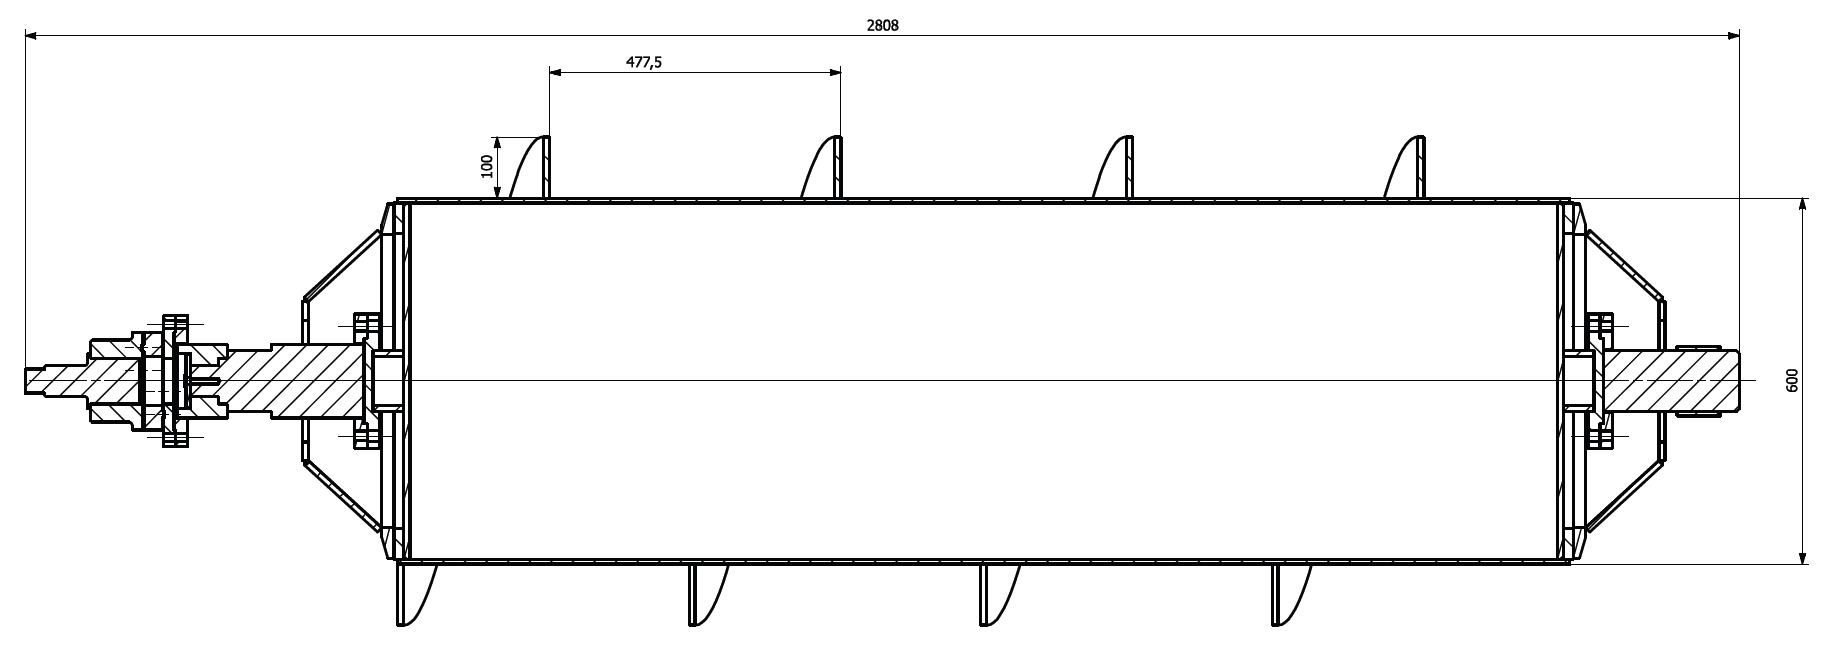
\includegraphics[width=\textwidth]{Archimedes_cross_section.png}
\end{RoyalFigure}

\subsubsection{PROPULSION SYSTEM MODEL}

The propulsion system is modeled and shown in Figure~\ref{fig:propulsionsystemmodel}. In this situation, an
electrical motor, drives a hydraulic pump. This electrical motor delivers a certain torque \gls{sym-tau}, where the
hydraulic pump demands a certain torque. This torque difference \gls{sym-Delta_tau} divided by the sum of inertia's and
integrated over time, translates to a certain rotational speed \gls{sym-omega}, with which this system turns. This
hydraulic pump generates a pressure \gls{sym-p}, which delivers energy to a hydraulic motor, which has a pressure drop,
or in other words converts this energy in a certain torque at a certain rotational speed. The pressure difference
\gls{sym-Delta_p}, between the hydraulic pump and motor, multiplied with the cross section, in which the hydraulic oil
flows, and divided with the total mass of hydraulic oil, integrated over time, results in a fluid velocity. This
hydraulic motor drives the Archimedes screws, which interact with the soil and generate a force which, which when total
friction and resistance is overcome translate to a velocity.

\newpage
\begin{RoyalFigure}[!htb, label=fig:propulsionsystemmodel]{DRIVE TRAIN BASED ON FIRST PRINCIPLE}
		\begin{tikzpicture}[auto, node distance=2.5cm,>=latex', align=center]
		% Placing the blocks
		\node [input, name=input] {};
		\node [block, below of=input] (Emotor) {\( E_{motor} \)};
		\node [left of=Emotor] (formEmotor) {\footnotesize{ \( \left. \gls{sym-tau} = \frac{\gls{sym-P}}{\gls{sym-omega}} \right\} \)}};
		\node [sum, below of=Emotor, yshift=-0.5cm, align=center] (sum1) {\( + \) \\ \( - \)};
		\node [block, right of=sum1, xshift=1cm] (deltaEmotor_Hpump) {\( \int\frac{\gls{sym-Delta_tau}}{\gls{sym-I}} dt\)};
		\node [block, below of=sum1] (Hpump) {\( H_{pump} \)};
		\node [left of=Hpump, xshift=-2cm] (formHpump) {\footnotesize{ \( \arraycolsep=1.4pt\def\arraystretch{1} \left. \begin{array}{r}
			\gls{sym-Q} = \gls{sym-v_f} \gls{sym-A_p} \\
			\gls{sym-Q} = \gls{sym-Q_i} - \gls{sym-Q_l} \\
			\gls{sym-tau} = \gls{sym-tau_i} + \gls{sym-tau_f} \\
			\gls{sym-Q_i} = D \gls{sym-omega} \\
			\gls{sym-tau_i} = D \gls{sym-Delta_p} \\
			\gls{sym-Q_l} = \gls{sym-K_HP}\gls{sym-Delta_p} \\
			\gls{sym-tau_f} = \left(\gls{sym-tau_0} + \gls{sym-K_TP}|\gls{sym-Delta_p}|\right) \text{tanh}\left(\frac{4 \gls{sym-omega}}{\gls{sym-omega_th}} \right) \\
			\gls{sym-K_HP}= \frac{\gls{sym-mu_n}}{\gls{sym-rho} \gls{sym-mu}} \frac{\gls{sym-rho_n} \gls{sym-omega_n} D}{\gls{sym-Delta_p_n}} \left(1 - \gls{sym-eta_Vn}\right)
			\end{array} \right\} \) }};
		\node [sum, below of=Hpump, yshift=-0.5cm, align=center] (sum2) {\( + \) \\ \( - \)};
		\node [block, right of=sum2, xshift=1cm] (deltaHpump_Emotor) {\( \int\frac{\gls{sym-Delta_p} \gls{sym-A_p}}{\gls{sym-m_f}} dt\)};
		\node [block, below of=sum2] (Hmotor) {\( H_{motor} \)};
		\node [sum, below of=Hmotor, yshift=-0.5cm, align=center] (sum3) {\( + \) \\ \( - \)};
		\node [left of=Hmotor, xshift=-2cm] (formHmotor) { \footnotesize{ \(\arraycolsep=1.4pt\def\arraystretch{1} \left. \begin{array}{r}
			\gls{sym-Q} = \gls{sym-v_f} \gls{sym-A_p} \\
			\gls{sym-Q} = \gls{sym-Q_i} + \gls{sym-Q_l} \\
			\gls{sym-tau} = \gls{sym-tau_i} - \gls{sym-tau_f} \\
			\gls{sym-Q_i} = D \gls{sym-omega} \\
			\gls{sym-tau_i} = D \gls{sym-Delta_p} \\
			\gls{sym-Q_l} = \gls{sym-K_HP}\gls{sym-Delta_p} \\
			\gls{sym-tau_f} = \left(\gls{sym-tau_0} + \gls{sym-K_TP}|\gls{sym-Delta_p}|\right) \text{tanh}\left(\frac{4 \gls{sym-omega}}{\gls{sym-omega_th}} \right) \\
			\gls{sym-K_HP}= \frac{\gls{sym-mu_n}}{\gls{sym-rho} \gls{sym-mu}} \frac{\gls{sym-rho_n} \gls{sym-omega_n} D}{\gls{sym-Delta_p_n}} \left(\frac{1}{\gls{sym-eta_Vn}} - 1\right)
			\end{array} \right\} \) }};
		\node [block, right of=sum3, xshift=1cm] (deltaHmotor_Propulsion) {\( \int\frac{\gls{sym-Delta_tau}}{\gls{sym-I}} dt\)};
		\node [block, below of=sum3] (Propulsion) {\( Propulsion \)};
		\node [left of=Propulsion, xshift=-2cm] (formHmotor) { \footnotesize{ \(\arraycolsep=1.4pt\def\arraystretch{1} \left. \begin{array}{r}
			\gls{sym-gamma_sw} = \gls{sym-g} (\gls{sym-rho_ds} - \gls{sym-rho_w}) \\
			\gls{sym-F_sn} = \gls{sym-gamma_sw} \frac{(2\gls{sym-r_a})^2}{\gls{sym-d_a}}\sin(\gls{sym-theta_s}-\gls{sym-theta_s}\cos(\gls{sym-theta_s})) \\
			\gls{sym-F_sn} = \gls{sym-p_sb} = \gls{sym-s_c} \gls{sym-c_sb} \gls{sym-N_c} + \gls{sym-s_q} \gls{sym-p_q} \gls{sym-N_q} + \gls{sym-s_gamma} \frac{1}{2} \gls{sym-gamma_sw} \gls{sym-w_a} \gls{sym-N_gamma} \\
			\gls{sym-N_q} = \frac{1 + \sin \gls{sym-phi_s}}{1 - \sin \gls{sym-phi_s}} \exp(\pi \tan \gls{sym-phi_s}) \\
			\gls{sym-N_c} = (\gls{sym-N_q} - 1)\cot \gls{sym-phi_s} \\
			\gls{sym-N_gamma} = 2(\gls{sym-N_q} - 1)\tan \gls{sym-phi_s} \\
			\gls{sym-s_q} = 1 + \frac{\gls{sym-w_a}}{\gls{sym-l_a}} \sin \gls{sym-phi_s} \\
			\gls{sym-s_c} = 1 + 0.2 \frac{\gls{sym-w_a}}{\gls{sym-l_a}} \\
			\gls{sym-s_gamma} = 1 - 0.3 \frac{\gls{sym-w_a}}{\gls{sym-l_a}} \\
			\gls{sym-V_sa} = \gls{sym-A_s} \gls{sym-l_a} \\
			\gls{sym-A_s} = \pi \gls{sym-r_a}^2(\gls{sym-theta_s} - \sin(\gls{sym-theta_s})\cos(\gls{sym-theta_s})) \\
			\gls{sym-s_a} = \gls{sym-r_a} \gls{sym-theta_s} \\
			\gls{sym-d_a} = \gls{sym-r_a}\left(1-\cos(\frac{\gls{sym-theta_s}}{2})\right) \\
			\gls{sym-F_b} = g \gls{sym-V_sa} \left(\gls{sym-rho_is} - \gls{sym-rho_w}\right)

			\end{array} \right\} \)} };
		\node [sum, below of=Propulsion, yshift=-0.5cm, align=center] (sum4) {\( + \) \\ \( - \)};
		\node [block, right of=sum4, xshift=1cm] (deltaForce) {\( \int\frac{\gls{sym-Delta_F}}{\gls{sym-m_cr}} dt\)};
		\node [block, below of=sum4] (Resistance) { \( F_{resistance} \) };

		\node [input, right of=deltaEmotor_Hpump] (p1) {};
		\node [input, above of=p1, yshift=-2.5mm] (p1a) {};
		\node [input, below of=p1, yshift=2.5mm] (p1b) {};

		\node [input, right of=deltaHpump_Emotor] (p2) {};
		\node [input, above of=p2, yshift=-2.5mm] (p2a) {};
		\node [input, below of=p2, yshift=2.5mm] (p2b) {};

		\node [input, right of=deltaHmotor_Propulsion] (p3) {};
		\node [input, above of=p3, yshift=-2.5mm] (p3a) {};
		\node [input, below of=p3, yshift=2.5mm] (p3b) {};

		\node [input, right of=deltaForce] (p4) {};
		\node [input, above of=p4, yshift=-2.5mm] (p4a) {};
		\node [input, below of=p4, yshift=2.5mm] (p4b) {};

		\node [right of=p4, xshift=-10mm] (output) {Dredgebot \\ speed};

		\draw [draw,->] (input) -- node [left] {\( \gls{sym-P} \) \\ \( [W] \)} (Emotor);
		\draw [->] (Emotor) -- node [left] {\( \gls{sym-tau} \) \\ \( [Nm] \)} (sum1);
		\draw [->] (Hpump) -- node [left] {\( \gls{sym-tau} \) \\ \( [Nm] \)} (sum1);
		\draw [->] (sum1) -- node {\( \gls{sym-Delta_tau} \) \\ \( [Nm] \)} (deltaEmotor_Hpump);
		\draw [-] (deltaEmotor_Hpump) -- node {\( \gls{sym-omega} \) \\ \( [rad/s] \)} (p1);
		\draw [-] (p1) -- (p1a);
		\draw [->] (p1a) -- ($ (Emotor.east)+(0,-0.25) $);
		\draw [-] (p1) -- (p1b);
		\draw [->] (p1b) -- ($ (Hpump.east)+(0,0.25) $);

		\draw [->] (Hpump) -- node [left] {$ p $ \\ $ [Pa] $} (sum2);
		\draw [->] (Hmotor) -- node [left] {$ p $ \\ $ [Pa] $} (sum2);
		\draw [->] (sum2) -- node {$ \gls{sym-Delta_p} $ \\ $ [Pa] $} (deltaHpump_Emotor);
		\draw [-] (deltaHpump_Emotor) -- node {$ v $ \\ $ [m/s] $} (p2);
		\draw [-] (p2) -- (p2a);
		\draw [->] (p2a) -- ($ (Hpump.east)+(0,-0.25) $);
		\draw [-] (p2) -- (p2b);
		\draw [->] (p2b) -- ($ (Hmotor.east)+(0,0.25) $);

		\draw [->] (Hmotor) -- node [left] {$ \gls{sym-tau} $ \\ $ [Nm] $} (sum3);
		\draw [->] (Propulsion) -- node [left] {$ \gls{sym-tau} $ \\ $ [Nm] $} (sum3);
		\draw [->] (sum3) -- node {$ \gls{sym-Delta_tau} $ \\ $ [Nm] $} (deltaHmotor_Propulsion);
		\draw [-] (deltaHmotor_Propulsion) -- node {$ \gls{sym-omega} $ \\ $ [rad/s] $} (p3);
		\draw [-] (p3) -- (p3a);
		\draw [->] (p3a) -- ($ (Hmotor.east)+(0,-0.25) $);
		\draw [-] (p3) -- (p3b);
		\draw [->] (p3b) -- ($ (Propulsion.east)+(0,0.25) $);

		\draw [->] (Propulsion) -- node [left] {$ F $ \\ $ [N] $} (sum4);
		\draw [->] (Resistance) -- node [left] {$ F $ \\ $ [N] $} (sum4);
		\draw [->] (sum4) -- node {$ \gls{sym-Delta_F} $ \\ $ [N] $} (deltaForce);
		\draw [-] (deltaForce) -- node {$ v $ \\ $ [m/s] $} (p4);
		\draw [-] (p4) -- (p4a);
		\draw [->] (p4a) -- ($ (Propulsion.east)+(0,-0.25) $);
		\draw [-] (p4) -- (p4b);
		\draw [->] (p4b) -- ($ (Resistance.east)+(0,0.25) $);
		\draw [->]	(p4) -- (output);

		\end{tikzpicture}
\end{RoyalFigure}
\newpage

\paragraph{A HYDRAULIC PUMP} is used to convert mechanical- to hydraulic energy is modeled after the, by
\citet{mathworks_mechanical_hydraulic_2016}, described model. In order to make a model based on first principle, the
hydraulic pump, should accept an variable fluid speed \( \gls{sym-v_f}(\cdot) \) and angular velocity of the electro
motor \gls{sym-omega}, whilst calculating a pressure gain \gls{sym-Delta_p} and needed torque \gls{sym-tau}. The flow
rate which is generated at the pump is equal to equation~\ref{eq:flow rate}. Where \gls{sym-A_p} is the cross-section of
the pipe and \gls{sym-v_f} is the average speed of the fluid, through that cross-section. Where \gls{sym-Q} is the net
volumetric flow rate.

\begin{equation}\label{eq:flow rate}
	\gls{sym-Q}(\gls{sym-v_f}) = \gls{sym-A_p} \gls{sym-v_f}
\end{equation}

\noindent The net volumetric flow rate obtained from equation~\ref{eq:flow rate} consists of an an ideal flow
\gls{sym-Q_i} where a leakage flow \gls{sym-Q_l} is subtracted, as is shown in equation~\ref{eq:pump flowrate}.

\begin{equation}\label{eq:pump flowrate}
	\gls{sym-Q}(\gls{sym-v_f}, \gls{sym-omega}) = \gls{sym-Q_i}(\gls{sym-omega}) - \gls{sym-Q_l}
\end{equation}

\noindent The ideal flow rate, needed by equation~\ref{eq:pump flowrate}, is generated by a displaced volume \( D \)
times the rotational speed \gls{sym-omega}. Which is shown in equation~\ref{eq:ideal flow rate}.

\begin{equation}\label{eq:ideal flow rate}
	\gls{sym-Q_i}(\gls{sym-omega}) = D \gls{sym-omega}
\end{equation}

\noindent Where the leakage flow rate compares to the Hagen-Poiseuille coefficient for laminar pipe flows
\gls{sym-K_HP}, which is computed for nominal parameters and multiplied with the pressure gain \gls{sym-Delta_p}.

\begin{equation}\label{eq:leak flow rate}
	\gls{sym-Q_l} = \gls{sym-K_HP}\gls{sym-Delta_p}
\end{equation}

\noindent In order to determine the pressure gain as a function of fluid speed and angular velocity,
equations \ref{eq:flow rate}, \ref{eq:pump flowrate}, \ref{eq:ideal flow rate} and \ref{eq:leak flow rate} can be
combined and rewritten in to equation~\ref{eq:dpp}.

\begin{equation}\label{eq:dpp}
	\gls{sym-Delta_p}(\gls{sym-v_f}, \gls{sym-omega}) = \frac{D \gls{sym-omega} - \gls{sym-A_p} \gls{sym-v_f}}{ \gls{sym-K_HP}}
\end{equation}

\noindent The Hagen-Poiseuille coefficient, needed in equation~\ref{eq:leak flow rate} and~\ref{eq:dpp}, is calculated
with the nominal viscosity \gls{sym-mu_n}, nominal density \gls{sym-rho_n} and the displacement volume \( D \). Divided
by the actual density \gls{sym-rho} and viscosity \gls{sym-mu}.

\begin{equation}
	\gls{sym-K_HP}= \frac{\gls{sym-mu_n}}{\gls{sym-rho} \gls{sym-mu}} \frac{\gls{sym-rho_n} \gls{sym-omega_n} D}{\gls{sym-Delta_p_n}} \left(1 - \gls{sym-eta_Vn}\right)
\end{equation}

\noindent In order for the pump to generate a flow a driving torque is required. The needed driving torque
\gls{sym-tau} consists of an ideal driving torque \gls{sym-tau_i} and a resistance, which is to be overcome, due to
friction \gls{sym-tau_f}.

\begin{equation}
	\gls{sym-tau}(\gls{sym-v_f}, \gls{sym-omega}) = \gls{sym-tau_i}(\gls{sym-v_f}, \gls{sym-omega}) + \gls{sym-tau_f}(\gls{sym-v_f}, \gls{sym-omega})
\end{equation}

\noindent While the ideal driving torque \gls{sym-tau_i} is also a function the displaced volume \( D \) times the
pressure gain from inlet to outlet \gls{sym-Delta_p}, as is shown in equation~\ref{ideal torque}.

\begin{equation}\label{ideal torque}
	\gls{sym-tau_i}(\gls{sym-v_f}, \gls{sym-omega}) = D \gls{sym-Delta_p}(\gls{sym-v_f}, \gls{sym-omega})
\end{equation}

\noindent The friction generated by the torque \gls{sym-tau_f} is calculated according to equation~\ref{eq:torque friction}.
In this equation, \gls{sym-tau_0} represent the no-load torque parameter and \gls{sym-omega_th} is the threshold angular
velocity for the pump-motor transition. The threshold angular velocity is an internally set fraction of the Nominal
shaft angular velocity parameter. The Friction torque vs pressure gain coefficient parameter \gls{sym-K_TP}.

\begin{equation}\label{eq:torque friction}
	\gls{sym-tau_f}(\gls{sym-v_f}, \gls{sym-omega}) = \left(\gls{sym-tau_0} + \gls{sym-K_TP}|\gls{sym-Delta_p}(\gls{sym-v_f}, \gls{sym-omega})|\right) \text{tanh}\left(\frac{4 \gls{sym-omega}}{\gls{sym-omega_th}} \right)
\end{equation}

\paragraph{A HYDRAULIC MOTOR} is used to convert hydraulic energy into mechanical energy. This actuator is modeled after
a \citet{mathworks_mechanical_hydraulic_2016}, described model. It receives feedback from the fluid velocity
\gls{sym-v_f} and the angular velocity \gls{sym-omega} of the propulsion system. It generates torque \gls{sym-tau} by
converting pressure \gls{sym-p}. The workings of a hydraulic pump and motor share much similarities, with some notable
differences related to the leakage flow. Were a pump subtracts the leakage flow it is added in this model. Since the
efficiency is an inverse of the pump.

\begin{equation}\label{eq:motor flowrate}
	\gls{sym-Q} = \gls{sym-Q_i} + \gls{sym-Q_l}
\end{equation}

\noindent In order to calculate a pressure drop as an function of fluid and angular velocity over the outlets, equations
\ref{eq:flow rate}, \ref{eq:motor flowrate}, \ref{eq:ideal flow rate} and \ref{eq:leak flow rate} can be combined and
rewritten in to equation \ref{eq:dpp motor}.

\begin{equation}\label{eq:dpp motor}
	\gls{sym-Delta_p}(\gls{sym-v_f}, \gls{sym-omega}) = \frac{\gls{sym-v_f} \gls{sym-A_p} - D \gls{sym-omega}}{ \gls{sym-K_HP}}
\end{equation}

\noindent In equation \ref{eq:dpp motor} the Hagen-Poiseuille coefficient for laminar pipe flows is calculated according
to equation \ref{eq:hagen}

\begin{equation}\label{eq:hagen}
	\gls{sym-K_HP}= \frac{\gls{sym-mu_n}}{\gls{sym-rho} \gls{sym-mu}} \frac{\gls{sym-rho_n} \gls{sym-omega_n} D}{\gls{sym-Delta_p_n}} \left(\frac{1}{\gls{sym-eta_Vn}} - 1\right)
\end{equation}

\noindent An other notable difference is that the net torque is lessened by the friction, as is shown in equation
\ref{eq:torque}. Where the ideal torque \( \gls{sym-tau_i}(v,\gls{sym-omega}) \)and torque generated by friction \(
\gls{sym-tau_f}(\gls{sym-v_f},\gls{sym-omega}) \) are calculated according to equation \ref{ideal torque} and \ref{eq:torque
friction}.

\begin{equation}\label{eq:torque}
	\gls{sym-tau}(\gls{sym-v_f},\gls{sym-omega}) = \gls{sym-tau_i}(\gls{sym-v_f},\gls{sym-omega}) - \gls{sym-tau_f}(\gls{sym-v_f},\gls{sym-omega})
\end{equation}

\subsection{SOIL DYNAMIC MODEL}

At this stage it is needed to model all interactions of a propulsion systems with a soil bed. According to
\citet{lotman_applicable_2009} the soil mechanics behind a moving process with Archimedes screws is similar to those of
track propulsion. The type of soil interaction can be modeled according to the rules of soil mechanics. The paragraphs
below are based on \citet{verruijt_soil_2007}. In the described model, the following simplifications are proposed: No
\gls{gls-dilatancy} behavior occurs, the displaced soil is completely replaced by the Archimedes screws. Thus, no build up
of soil is created at the sides of a screw, due to a bulldozer effect.

In order to generate a forward thrust, an Archimedes screw has to be (partial) submerged in the soil. The depth of
submersion depends on the weight and buoyancy of the displaced volume or the soil bearing capacity. The distributed load
\gls{sym-p_sb} representing the crawler, is applied at a certain depth \gls{sym-d_a}. Where the normal force working on
the submerged surface of an Archimedes screw are in equilibrium with the weight and buoyancy of a crawler.

It is important to note that the material of a soil bed, determines how the sinkage depth is calculated. When the soil
bed consists of silt-like material it is assumed that the soil bearing capacity goes to zero, because the cohesion
\gls{sym-c_sb} will lessen, combined with a smaller difference between a specific in-situ weight of silt
\gls{sym-rho_is} compared to water \gls{sym-rho_w}, resulting in a small specific in-situ weight \gls{sym-gamma_sw}.
Setting all terms in the Brinch-Hansen equation~\ref{eq:Brinch-Hansen} to zero. Which allow for a simplification of the
sinkage depth calculation. Which does now, only consist of a downwards force, due to weight and a buoyancy force, due to
the replaced soil.

\begin{RoyalFigure}[!htb, label=fig:F_n]{NORMAL FORCES WORKING ON PARTIAL SUBMERGED CYLINDER}
		\begin{tikzpicture}
		\tikzstyle{loosely dashdotted}= [dash pattern=on 3pt off 4pt on \the\pgflinewidth off 4pt,line width=0.05mm]
		\def\h{1};
		\def\r{2};
		\def\f{1.05};
		\draw (0,0) circle (\r);

		\draw [RoyalLightGrey](-4.5,\h*-1) -- (4.5,\h*-1);
		\coordinate (x0) at (0,0);
		\coordinate (x0r) at (\r,0);
		\coordinate (x1) at ({((\r^2)-(\h^2))^(1/2)},{\h*-1});
		\coordinate (x2) at ({-1*((\r^2)-(\h^2))^(1/2)},{\h*-1});
		\coordinate (x3) at ($(x0)!0.25!(x1)$);
		\coordinate (x4) at ($(x0)!1.1!(x1)$);
		\coordinate (m0) at (0,\r);
		\coordinate (m1) at (\r+0.5, \r);
		\coordinate (m2) at (\r, 0);
		\coordinate (m3) at (\r+0.5,0);
		\coordinate (m4) at ({((\r^2)-(\h^2))^(1/2)},\h*-1);
		\coordinate (m5) at (\r+0.5,\h*-1);
		\coordinate (m6) at (0,\r*-1);
		\coordinate (m7) at (\r+0.5,\r*-1);

		\draw (x0) -- (x1);

		\fill[pattern=crosshatch dots, pattern color=RoyalRed!25] (-4.5,\h*-1) rectangle (4.5,-3);
		\draw [RoyalRed,fill=RoyalRed!10,line width=0.25mm,rotate=-150] (x2) arc (0:120:\r) -- (x2);

		\draw [loosely dashdotted] ({\r*\f*-1},0) -- ({\r*\f},0);
		\draw [loosely dashdotted] (0,{\r*\f*-1}) -- (0,{\r*\f});
		\node (Soil) at (-3,-2.5) {Soil bed};
		\node (Water) at (-3,1.5) {Water};
		\node (normal) at (-1.5,-2.5) {\gls{sym-F_sn}};
		\node (load) at (-0.75,-0.75) {\gls{sym-p_sb}};
		\draw [{Latex[length=2mm,width=1mm]}-{Latex[length=2mm,width=1mm]}, rotate=-90,line width=0.05mm](x3) arc (60:0:\r/4);
		\node (theta) at (0.75,-0.75) {\gls{sym-theta_s}};
		\draw [line width=0.05mm](m4) -- (m5);
		\draw [line width=0.05mm](m6) -- (m7);
		\draw [{Latex[length=2mm,width=1mm]}-{Latex[length=2mm,width=1mm]},line width=0.05mm] ([shift={(-0.125,0)}]m5) --([shift={(-0.125,0)}]m7) node[midway, right] {\gls{sym-d_a}};

		\foreach \x in {210,215,...,265} \draw[-{Latex[length=2mm,width=1mm]}] (\x:{\r+(0.75*((\x-210)/60))+0.1}) -- (\x:\r);
		\foreach \x in {210,215,...,265} \draw[-{Latex[length=2mm,width=1mm]}] (\x:{\r-(0.75*((\x-210)/60))-0.1}) -- (\x:\r);
		\foreach \x in {330,325,...,270} \draw[-{Latex[length=2mm,width=1mm]}] (\x:{\r+(-0.75*((\x-330)/60))+0.1}) -- (\x:\r);
		\foreach \x in {330,325,...,270} \draw[-{Latex[length=2mm,width=1mm]}] (\x:{\r-(-0.75*((\x-330)/60))-0.1}) -- (\x:\r);
		\end{tikzpicture}
\end{RoyalFigure}

When the crawler operates in an environment with a sand-like soil bed, the load \gls{sym-p_sb}, shown in
Figure~\ref{fig:bearing_capacity}, can be set equal to the normal force \gls{sym-F_sn} working on a certain point at a
submerged cross section of an Archimedes screw, as is shown in Figure~\ref{fig:F_n}. For silt and sand calculations, a
specific weight difference \gls{sym-gamma_sw} between soil and water can be expressed as equation~\ref{eq:submerged
weight}, were \gls{sym-rho_is} is the in-situ density of the drained soil, \gls{sym-rho_w} of water and \gls{sym-g} the
acceleration due to gravity.

\begin{equation}\label{eq:submerged weight}
	\gls{sym-gamma_sw} = \gls{sym-g} (\gls{sym-rho_is} - \gls{sym-rho_w})
\end{equation}

\citet{miedema_slurry_2016} shows that the normal forces working on a pipe from the inside can be calculated with
equation \ref{eq:miedema_F_n_pipe}. He multiplies the density of undrained soil over a pipe length \gls{sym-Delta_L},
where a fraction of the density between soil and water \( \gls{sym-Re_sd} = \frac{\gls{sym-rho_ds}}{\gls{sym-rho_w}} - 1
\) combined with a volumetric bed concentration fraction \gls{sym-C_vb}, which combined can be describes as an in-situ
specific weight difference \gls{sym-gamma_sw}, found in equation~\ref{eq:submerged weight}. This is multiplied with a
term that describes the contact face, determined with a sinkage angle \gls{sym-theta_s} and a pipe diameter
\gls{sym-d_p}. This normal forces working on a pipe from inside-out can be translated to normal forces working on an
Archimedes screw from outside in, as shown in Figure~\ref{fig:F_n} can be calculated with equation~\ref{eq:normal}. Were
equation~\ref{eq:miedema_F_n_pipe} is rewritten, combining multiple terms in the in-situ specific weight and dividing
the total normal force \gls{sym-F_n} with the length of an Archimedes screw and its penetration depth.

\begin{equation}\label{eq:miedema_F_n_pipe}
		\gls{sym-F_n} = \gls{sym-rho_is} \gls{sym-g} \gls{sym-Delta_L} \gls{sym-Re_sd} \gls{sym-C_vb} \frac{\gls{sym-d_p}^2}{2}\sin(\gls{sym-theta_s}-\gls{sym-theta_s}\cos(\gls{sym-theta_s}))
\end{equation}

\begin{equation}\label{eq:normal}
	\gls{sym-F_sn} = \gls{sym-gamma_sw} \frac{(2\gls{sym-r_a})^2}{\gls{sym-d_a}}\sin(\gls{sym-theta_s}-\gls{sym-theta_s}\cos(\gls{sym-theta_s}))
\end{equation}

\begin{RoyalFigure}[!htb, label=fig:bearing_capacity]{PRANDTL BEARING CAPACITY AND STRESS ZONES}
		\begin{tikzpicture}
		\point{a}{0.3}{3};
		\point{aa}{-0.1}{2.9};
		\point{b}{5}{3};
		\point{bb}{5}{2.7};
		\point{c}{10}{3};
		\point{cc}{10}{2.7};
		\point{d}{14.7}{3};
		\point{e}{2}{5};
		\point{f}{7}{6};
		\point{g}{13}{5};
		\point{h}{2.5}{2.25};
		\point{i}{12.5}{2.25};
		\point{j}{7.5}{2.25};
		\point{k}{5}{1.75};
		\point{l}{10}{1.75};
		\beam{3}{a}{d}[0][0];
		\lineload{2}{a}{b}[1][1][0.125];
		\lineload{2}{bb}{cc}[2][2][0.125];
		\lineload{2}{c}{d}[1][1][0.125];
		\snotation{1}{e}{\( \gls{sym-p_q} = \gamma \gls{sym-d_a} \)}[above];
		\snotation{1}{f}{\gls{sym-p_sb}}[above];
		\snotation{1}{g}{\( \gls{sym-p_q} = \gamma \gls{sym-d_a} \)}[above];
		\snotation{1}{h}{\( \mathrm{I} \)}[above];
		\snotation{1}{i}{\( \mathrm{I} \)}[above];
		\snotation{1}{j}{\( \mathrm{III} \)}[above];
		\snotation{1}{k}{\( \mathrm{II} \)}[above];
		\snotation{1}{l}{\( \mathrm{II} \)}[above];
		\snotation{1}{aa}{\gls{sym-d_a}};
		\draw (0.3,3) -- (2.5,2) -- (5,3);
		\draw (5,3) -- (7.5,2) -- (10,3);
		\draw (10,3) -- (12.5,2) -- (14.7,3);
		\draw (2.5,2) .. controls (4,1.5) and (6,1.5) .. (7.5,2);
		\draw (7.5,2) .. controls (9,1.5) and (11,1.5) .. (12.5,2);
		\draw [fill=RoyalRed!20] (0.3,3) -- (0.3,3.3) -- (5,3.3) -- (5,3) -- cycle;
		\draw [fill=RoyalRed!20] (10,3) -- (10,3.3) -- (14.7,3.3) -- (14.7,3) -- cycle;
		\end{tikzpicture}
\end{RoyalFigure}

There are three situations which can occur; Firstly the soil bed has enough strength to carry a crawler. In this
situation the speed of a crawler is a direct function of the pitch of the vanes. Secondly, the weight of a crawler is
higher than the soil bed capacity and the Archimedes screws sink, partial, into the undrained soil, till there exist an
equilibrium between load \gls{sym-p_sb} and the submerged weight of the soil \gls{sym-gamma_sw}, as is
illustrated in Figure~\ref{fig:bearing_capacity}. The last case builds on the previous situation, only here are the
Archimedes screws completely surrounded by soil.

Figure~\ref{fig:bearing_capacity} shows the resulting situation of the bearing capacity and the stress zones underneath
the loads \gls{sym-p_sb} and \gls{sym-p_q}. \textbf{Zone I} is an area were the horizontal principle stress
\gls{sym-sigma_H} is greater than the vertical principle stress \gls{sym-sigma_V}. Whilst \textbf{zone II} is a
transition zone between \textbf{I} and \textbf{III}. Where in \textbf{zone III} the vertical principle stress, which is
equal to \gls{sym-p_sb}, is greater than horizontal principle stress, as shown in equation \ref{eq:bigger v instead of h stress}.

\begin{equation}\label{eq:bigger v instead of h stress}
	\gls{sym-sigma_H} < \gls{sym-sigma_V} = \gls{sym-p_sb}
\end{equation}

\noindent A maximum allowable load of \gls{sym-p_sb} is calculated according to the method proposed by
Brinch-Hansen. Which gives an indication when the soil bed starts to give way and deform. Where \gls{sym-p_sb} can
be set equal to the normal forces acting at a certain point \gls{sym-F_sn}, as show in equation~\ref{eq:normal}.

\begin{equation}\label{eq:Brinch-Hansen}
	\gls{sym-F_sn} = \gls{sym-p_sb} = \gls{sym-s_c} \gls{sym-c_sb} \gls{sym-N_c} + \gls{sym-s_q} \gls{sym-p_q} \gls{sym-N_q} + \gls{sym-s_gamma} \frac{1}{2} \gls{sym-gamma_sw} \gls{sym-w_a} \gls{sym-N_gamma}
\end{equation}

\noindent Were \gls{sym-N_q}, \gls{sym-N_c} and \gls{sym-N_gamma} are dimensionless constants and are given by
equations:~\ref{eq:Nq},~\ref{eq:Nc} and~\ref{eq:Ngamma}. In these equations the angle of internal friction
\gls{sym-phi_s} and \gls{sym-c_sb} is the cohesion of the soil. Which both can be obtained through laboratory tests.

\begin{equation}\label{eq:Nq}
	\gls{sym-N_q} = \frac{1 + \sin \gls{sym-phi_s}}{1 - \sin \gls{sym-phi_s}} \exp(\pi \tan \gls{sym-phi_s})
\end{equation}

\begin{equation}\label{eq:Nc}
		\gls{sym-N_c} = (\gls{sym-N_q} - 1)\cot \gls{sym-phi_s}
\end{equation}

\begin{equation}\label{eq:Ngamma}
		\gls{sym-N_gamma} = 2(\gls{sym-N_q} - 1)\tan \gls{sym-phi_s}
\end{equation}

\noindent And the shape factors \gls{sym-s_q}, \gls{sym-s_c} and \gls{sym-s_gamma} are calculated using
equations:~\ref{eq:Sq},~\ref{eq:Sc} and~\ref{eq:Sgamma}; Where \gls{sym-w_a} and \gls{sym-l_a} are the dimensions of
width and length.

\begin{equation}\label{eq:Sq}
	\gls{sym-s_q} = 1 + \frac{\gls{sym-w_a}}{\gls{sym-l_a}} \sin \gls{sym-phi_s}
\end{equation}

\begin{equation}\label{eq:Sc}
	\gls{sym-s_c} = 1 + 0.2 \frac{\gls{sym-w_a}}{\gls{sym-l_a}}
\end{equation}

\begin{equation}\label{eq:Sgamma}
	\gls{sym-s_gamma} = 1 - 0.3 \frac{\gls{sym-w_a}}{\gls{sym-l_a}}
\end{equation}

\noindent Since the width of the Archimedes screw is a function of the sinkage depth, an approximation is made When a
load is placed on the soil, and the bearing capacity proofs to be insufficient; That load will sink into the soil bed
increasing the depth \gls{sym-d_a}. Because the sinkage depth increases, the bearing capacity will also increase; Until
an equilibrium with the load, buoyancy and bearing capacity exists. This depth can be found through an iterative
process. This is needed because the width \gls{sym-w_a} of an Archimedes screw changes as a function of the depth.

\begin{RoyalFigure}[!htb, label=fig:cylinder]{DISPLACED VOLUME OF A PARTIAL SUBMERGED CYLINDER}
		\begin{tikzpicture}
		\tikzstyle{loosely dashdotted}= [dash pattern=on 3pt off 4pt on \the\pgflinewidth off 4pt,line width=0.05mm]
		\def\h{1};
		\def\r{2};
		\def\f{1.05};
		\draw (0,0) circle (\r);

		\draw [RoyalLightGrey](-4.5,\h*-1) -- (4.5,\h*-1);
		\coordinate (x0) at (0,0);
		\coordinate (x0r) at (\r,0);
		\coordinate (x1) at ({((\r^2)-(\h^2))^(1/2)},{\h*-1});
		\coordinate (x2) at ({-1*((\r^2)-(\h^2))^(1/2)},{\h*-1});
		\coordinate (x3) at ($(x0)!0.25!(x1)$);
		\coordinate (x4) at ($(x0)!1.1!(x1)$);
		\coordinate (m0) at (0,\r);
		\coordinate (m1) at (\r+0.5, \r);
		\coordinate (m2) at (\r, 0);
		\coordinate (m3) at (\r+0.5,0);
		\coordinate (m4) at ({((\r^2)-(\h^2))^(1/2)},\h*-1);
		\coordinate (m5) at (\r+0.5,\h*-1);
		\coordinate (m6) at (0,\r*-1);
		\coordinate (m7) at (\r+0.5,\r*-1);

		\draw (x0) -- (x1);
		\draw (x0) -- (x2);
		\fill[pattern=crosshatch dots, pattern color=RoyalRed!20] (-4.5,\h*-1) rectangle (4.5,-3);
		\draw [RoyalRed,fill=RoyalRed!10,line width=0.25mm,rotate=-150] (x2) arc (0:120:\r) -- (x2);

		\draw [loosely dashdotted] ({\r*\f*-1},0) -- ({\r*\f},0);
		\draw [loosely dashdotted] (0,{\r*\f*-1}) -- (0,{\r*\f});
		\draw [{Latex[length=2mm,width=1mm]}-{Latex[length=2mm,width=1mm]}, rotate=-90,line width=0.05mm](x3) arc (60:0:\r/4);
		\draw [{Latex[length=2mm,width=1mm]}-{Latex[length=2mm,width=1mm]}, rotate=-150,line width=0.05mm](x4) arc (120:0:\r*1.1);
		\node (theta) at (0.75,-0.75) {\gls{sym-theta_s}};
		\node (As) at (0.5,-1.30) {\gls{sym-A_s}};
		\node (S) at (-1.3,-2) {\gls{sym-s_a}};
		\node (Soil) at (-2.5,-2.5) {Soil bed};
		\node (Water) at (-2.5,1.5) {Water};
		\node (rhoS) at (3.5, -2.5) {\gls{sym-rho_is}};
		\node (rhoW) at (3.5, 1.5) {\gls{sym-rho_w}};
		\draw [line width=0.05mm](m0) -- (m1);
		\draw [line width=0.05mm](m2) -- (m3);
		\draw [line width=0.05mm](m4) -- (m5);
		\draw [line width=0.05mm](m6) -- (m7);
		\draw [{Latex[length=2mm,width=1mm]}-{Latex[length=2mm,width=1mm]},line width=0.05mm] ([shift={(-0.125,0)}]m1) --([shift={(-0.125,0)}]m3) node[midway, right] {\gls{sym-r_a}};
		\draw [{Latex[length=2mm,width=1mm]}-{Latex[length=2mm,width=1mm]},line width=0.05mm] ([shift={(-0.125,0)}]m3) --([shift={(-0.125,0)}]m5) node[midway, right] {\gls{sym-h}};
		\draw [{Latex[length=2mm,width=1mm]}-{Latex[length=2mm,width=1mm]},line width=0.05mm] ([shift={(-0.125,0)}]m5) --([shift={(-0.125,0)}]m7) node[midway, right] {\gls{sym-d_a}};
		\end{tikzpicture}
\end{RoyalFigure}

\noindent The displaced volume \gls{sym-V_sa}of a surface area in the soil \gls{sym-A_s} on a submerged cross section,
show in Figure~\ref{fig:cylinder}, throughout the complete length \gls{sym-l_a} of an Archimedes screw, as is shown in
equation~\ref{eq:volume}.

\begin{equation}\label{eq:volume}
	\gls{sym-V_sa} = \gls{sym-A_s} \gls{sym-l_a}
\end{equation}

\noindent Where the sink angle \gls{sym-theta_s} is related to the surface area in the soil \gls{sym-A_s} by
equation~\ref{eq:as}.

\begin{equation}\label{eq:as}
	\gls{sym-A_s} = \pi \gls{sym-r_a}^2(\gls{sym-theta_s} - \sin(\gls{sym-theta_s})\cos(\gls{sym-theta_s}))
\end{equation}

\noindent The total arc length in contact with the soil can be calculate by multiplying the radius \gls{sym-r_a}
multiplied with the sink angle \gls{sym-theta_s}, as is shown in equation~\ref{eq:s}

\begin{equation}\label{eq:s}
	\gls{sym-s_a} = \gls{sym-r_a} \gls{sym-theta_s}
\end{equation}

\noindent Where the sinkage depth \gls{sym-d_a} can be obtained with equation~\ref{eq:d_a}. Where \gls{sym-r_a} [m]
is the radius of an Archimedes screw.

\begin{equation}\label{eq:d_a}
	\gls{sym-d_a} = \gls{sym-r_a}\left(1-\cos(\frac{\gls{sym-theta_s}}{2})\right)
\end{equation}

Because there are multiple interdependent variables in the equations~\ref{eq:submerged weight} through~\ref{eq:d_a}, the
sinkage depth needs to be determined numerically. The model for bearing capacity vs sinkage depth allows for a quick
exploration which gives an impression how deep a crawler will sink in different soil types, before settling. In
Figure~\ref{fig:sinkage depths} the bearing capacity is plotted against the sinkage depth. The source code for these
calculations can be found in Appendix~\ref{app:crawler bearing cap}. It is clear that that silt, with a sinkage of
\SI{135}{\milli\meter}, offers less bearing capacity compared to sand \SI{18}{\milli\meter} and clay, either loosly
\SI{45}{\milli\meter} or densly packed \SI{11}{\milli\meter}

\begin{RoyalFigure}[!htb, label=fig:sinkage depths]{SINKAGE DEPTH}
	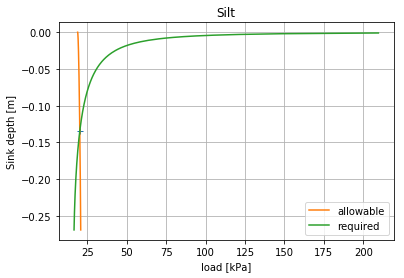
\includegraphics[width=0.25\textwidth,trim=2 2 2 2,clip]{sinkage_silt.png}
	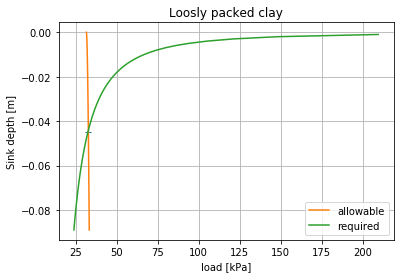
\includegraphics[width=0.25\textwidth,trim=2 2 2 2,clip]{sinkage_looslypackedclay.png}
	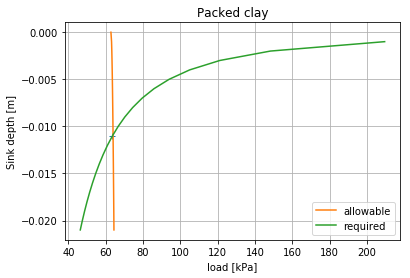
\includegraphics[width=0.25\textwidth,trim=2 2 2 2,clip]{sinkage_clay.png}
	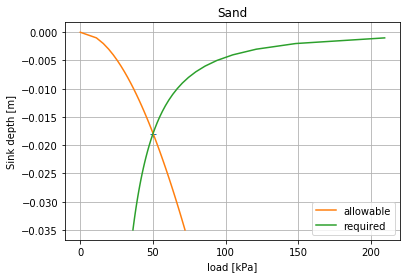
\includegraphics[width=0.25\textwidth,trim=2 2 2 2,clip]{sinkage_sand.png}
\end{RoyalFigure}

The sinkage depth is needed to determine friction losses between screw and soil. \citet{rajapakse_geotechnical_2011}
describe that Kolk and van der Velde developed a method to determine skin friction considering cohesion as well as
effective stress. Where \gls{sym-F_u} is the ultimate skin friction, \gls{sym-alpha_sf} is a skin friction coefficient,
obtained using the correlations provide by Kolk and Van der Velde. The parameter \gls{sym-alpha_sf} is based on a ratio
between both on cohesion \gls{sym-c_sb} and effective stress \gls{sym-sigma_prime}, to obtain \gls{sym-alpha_sf}.
\gls{sym-c_u} is the undrained shear strength or cohesion properties of the soil.

\begin{equation}\label{eq:f_ult}
	\gls{sym-F_u} = \gls{sym-alpha_sf} \gls{sym-c_u}
\end{equation}

\noindent The total skin friction \gls{sym-F_s} for a certain area is given by equation~\ref{eq:total skin friction}.
Where \gls{sym-F_u} is obtained with equation~\ref{eq:f_ult} and  \gls{sym-A_a}, which can be determine by~
\ref{eq:total skin friction}.

\begin{equation}\label{eq:total skin friction}
	\gls{sym-F_s}  = \gls{sym-F_u} \gls{sym-A_a}
\end{equation}

\noindent The effective stress \gls{sym-sigma_prime} needed to determine  \gls{sym-alpha_sf}, can be found with
equation~\ref{eq:sigmaprime}. Here \gls{sym-m_cr_prime} is the buoyancy corrected weight of a crawler, which can be
expressed as \( \gls{sym-m_cr} - \frac{\gls{sym-F_crb}}{\gls{sym-g}} \). Where \gls{sym-F_crb} is given as the upwards
force generated in water due to a volumetric displacement of that water compared to the air filled chambers in the
crawler.

\begin{equation}\label{eq:sigmaprime}
	\gls{sym-sigma_prime} = \frac{\gls{sym-m_cr_prime}}{2 \gls{sym-A_a} }
\end{equation}

\noindent The surface in contact with the soil \gls{sym-A_a} is an arc length \gls{sym-s_a}, calculated in
equation~\ref{eq:s}, multiplied with the length of an Archimedes screw.

\begin{equation}\label{eq:contact surface}
	\gls{sym-A_a}  = \gls{sym-s_a} \gls{sym-l_a}
\end{equation}

The maximum allowable thrust which can be generated, can be calculated by the soil characteristics and the geometry of
the propulsion geometry. This thrust determines how fast a crawler moves and should overcome the drag-force through the
water. A maximum allowable thrust, is the horizontal stress at which passive soil failure occurs. This can be determine
with Rankine theory. Because movement occurs in undrained situation, the cohesion \gls{sym-c_sb} is equal to the
undrained shear strength \gls{sym-c_u} and the internal friction angle \gls{sym-phi_s} can be set equal to \( 0 \). In
effect simplifying equation~\ref{eq:horizontal stress} to~\ref{eq:max horizontal stress}.

\begin{equation}\label{eq:horizontal stress}
	\gls{sym-sigma_H} = \gls{sym-N_phi} \gls{sym-sigma_V} + 2\gls{sym-c_sb}\sqrt{\gls{sym-N_phi}}
\end{equation}

\begin{equation}
	\gls{sym-N_phi} = \frac{1 + \sin \gls{sym-phi_s}}{1 - \sin \gls{sym-phi_s}}
\end{equation}

\begin{equation}\label{eq:max horizontal stress}
	\gls{sym-sigma_H} = \gls{sym-sigma_V} + 2\gls{sym-c_u}
\end{equation}

An other factor that is depended on the penetration depth \gls{sym-d_a} is, a generated buoyancy. When these screws are
submerged in the soil, a resulting buoyancy force will exists, as a result of the displaced soil.
\citet{lotman_applicable_2009} describes the buoyancy force as depicted in equation~\ref{eq:buoyancy force}. In this
equation \gls{sym-g} is the gravitational constant and multiplied with the displaced volume \gls{sym-V_sa} and specific
weight difference between the soil and water, or in other words the specific weight difference  \gls{sym-gamma_sw},
found in equation~\ref{eq:submerged weight}.

\begin{equation}\label{eq:buoyancy force}
	\gls{sym-F_b} = \gls{sym-V_sa} \gls{sym-gamma_sw}
\end{equation}

\subsection{DREDGE MODEL}

During coverage travel the maximum speed \(\max \gls{sym-v_k}\) is limited against the performance of the dredging
system, see Note~\ref{assumption_dredge_speed}. When the crawler is in this state the \gls{gls-draghead} is lowered and
the projected front of this head is seen as the entrance for the \gls{gls-dredgeline} system. This sytem transports the
\gls{gls-slurry} to a \gls{gls-hopper} located above water. Transported \gls{gls-slurry} behave in reality as
\gls{gls-Bingham-plastic}s. Difficult to get moving, but once transportation is in a steady-state the assumption for
this paper is made that it behaves as regular Newtonian fluid.

There are two possible bottlenecks in this dredging system as a whole, one is the throughput in the dredge mouth, due to
its physical dimensions and transport performance of the auger, while the second is the hydraulic system. The throughput
of the system is

\import{resources/equations/}{v_s}
\import{resources/equations/}{v_p}
\import{resources/equations/}{p_s}
\import{resources/equations/}{p_v}
\import{resources/equations/}{p_i}
\import{resources/equations/}{p_ro}
\import{resources/equations/}{p_sm}
\import{resources/equations/}{p_rp}
\import{resources/equations/}{labda}
\import{resources/equations/}{Re}
\import{resources/equations/}{psi}
\import{resources/equations/}{c_t}
\import{resources/equations/}{F_r}
\import{resources/equations/}{p_p}
\import{resources/equations/}{p_man}




\subsection{STEERING MODEL}

The kinematic model of the crawler is comparable with a skid-steering model. Meaning that the crawler turns around its
axis by changing the translational velocity \gls{sym-v} of a single Archimedes screw, relative to the other. If both
screws, move with the same velocity, the crawler will travel in a straight line. This is a challenge in its own right,
as slippage of a screw is bound to occur, resulting in a difference between the input signal, which is the rotational
velocity \gls{sym-omega}, and the translational velocity of that screw. Assuming that the earlier described motion and
soil dynamic models, will compensate for occurring slippage and other drive-train characteristics, a model can be
described on a 2-dimensional space as a differential drive. Which is a very simple driving mechanism.

\begin{RoyalFigure}[!htb, label=fig:difdrivekinetics]{DIFFERENTIAL DRIVE KINEMATICS~\cite{klancar_wheeled_2017}}
	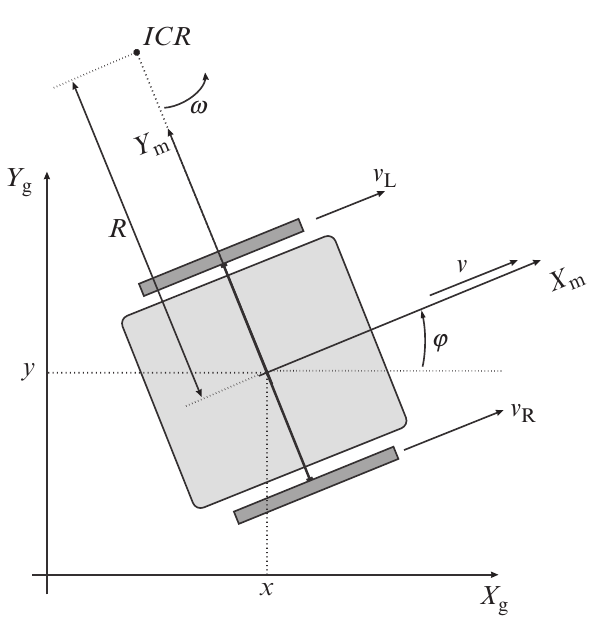
\includegraphics[height=5cm,trim=2 2 2 2,clip]{difdrivekinetics.png}
\end{RoyalFigure}

Considering Figure~\ref{fig:difdrivekinetics} it is possible to determine the rotation \gls{sym-psi} and tangential
velocity \gls{sym-v} of the crawler on the instantaneous radius \gls{sym-R_t} with the center ICR. \gls{sym-L} is
defined as the distance between the two screws and \gls{sym-v_L} and \gls{sym-v_R} are the translational velocities for
the left and right screw. \gls{sym-omega} is the angle between the global coordinate frame \( (X_g, Y_g) \) and the
moving frame attached to the center of mass of the crawler \( (X_m, Y_m) \).

\begin{equation}\label{eg:left}
	\gls{sym-omega} = \frac{\gls{sym-v_L}}{\gls{sym-R_t} - \frac{\gls{sym-L}}{2}}
\end{equation}

\begin{equation}\label{eg:right}
	\gls{sym-omega} = \frac{\gls{sym-v_R}}{\gls{sym-R_t} + \frac{\gls{sym-L}}{2}}
\end{equation}

\nodindent From where \gls{sym-omega} and \gls{sym-R_t} are expressed as follows:

\begin{equation}\label{eq:omega_t}
	\gls{sym-omega} = \frac{\gls{sym-v_R} - \gls{sym-v_L}}{\gls{sym-L}}
\end{equation}

\begin{equation}\label{eq:R_t}
	\gls{sym-R_t} = \frac{\gls{sym-L}}{2}\frac{\gls{sym-v_R} + \gls{sym-v_L}}{\gls{sym-v_R} - \gls{sym-v_L}}
\end{equation}

\noindent The translational tangential velocity of the crawler \gls{sym-v} is then calculated as:

\begin{equation}\label{eq:v_crawler}
	\gls{sym-v} = \gls{sym-omega} \gls{sym-R_t} = \frac{\gls{sym-v_R} + \gls{sym-v_L}}{2}
\end{equation}

\noindent using the above established relations a crawler local coordinates can be expressed as:

\begin{equation}\label{eq:local_frame}
	\left[\begin{array}{c}
		\dv{\gls{sym-x}}{t} \\
		\dv{\gls{sym-y}}{t} \\
		\dv{\gls{sym-psi}}{t}
	\end{array}\right] = \left[\begin{array}{cc}
		\frac{1}{2} & \frac{1}{2} \\
		0 & 0 \\
		-\frac{1}{\gls{sym-L}} & \frac{1}{\gls{sym-L}}
	\end{array}\right] \left[\begin{array}{c}
	  \gls{sym-v_L} \\
		\gls{sym-v_R}
	\end{array}\right]
\end{equation}


\section{CONTROLLER}\label{sec:controller}

\subsection{THE WORLD}

\subsection{A VESSEL}

\subsection{THE CAPTAIN}

\subsection{THE NAVIGATOR}


\subsection{A BOATSWAIN}
The boatswain is responsible for execution of the different tasks. A crawler has four states of operation, namely:
normal travel, dredging coverage travel, stationary dredging and standstill. These, and their transitions are depicted
in diagram \ref{fig:stateoperating}. These state dictate the maximum travel speed \gls{sym-x_k}. During normal travel, a
crawler moves from a start location to its goal, its traveling speed limited by the  maximum allowable power
delivered to the propulsion system.

\begin{RoyalFigure}[!htb, label=fig:stateoperating]{STATE OPERATIONS}
	\resizebox{9cm}{!}{
		\begin{tikzpicture}[->,>=stealth',shorten >=1pt,auto,node distance=3.5cm,
		semithick, every state/.style={minimum size=3cm, align=center}]

		\node[initial,state,fill=RoyalLightGrey!10] (standstill) {Standstill};
		\node[state,fill=RoyalLightGrey] (coverage) [right of=standstill, yshift=3cm, xshift=2cm] {Coverage dredging};
		\node[state,fill=RoyalLightGrey] (travel) [below of=coverage, xshift=-2cm, yshift=-2cm] {Travel};
		\node[state,fill=RoyalLightGrey] (localized) [left of=travel, yshift=-2cm, xshift=-2cm] {Localized dredging};
		\node (exit) [left of=standstill, xshift=20mm,yshift=20mm]	{exit};

		\path (standstill) edge [bend right] (travel);
		\path (travel) edge [bend right] (standstill);

		\path (localized) edge [bend right] (travel);
		\path (standstill) edge [bend right] (localized);
		\path (localized) edge [bend right] (standstill);

		\path (standstill) edge [bend right=10] (coverage);
		\path (coverage) edge [bend right=30] (standstill);

		\path (travel) edge [bend right] (coverage);
		\path (coverage) edge [bend right=10] (travel);

		\path (standstill) edge (exit);
		\end{tikzpicture}}
\end{RoyalFigure}

\subsubsection{COVERAGE DREDGING}

\subsubsection{TRAVEL}

\subsubsection{LOCALIZED DREDGING}
